\documentclass[a4paper,12pt]{article} % тип документа

% Поля страниц
\usepackage[left=2.5cm,right=2.5cm,top=1.5cm,bottom=2cm,bindingoffset=0cm]{geometry}
    
% Отступ после заголовка
\usepackage{indentfirst}

% Картинки
\usepackage{graphicx}
\graphicspath{{images/}}
\usepackage{placeins}

% Таблицы
\usepackage{booktabs}
% \usepackage{floatrow}
\usepackage{subcaption}

% Русский язык
\usepackage{cmap}  % поиск в PDF
\usepackage{mathtext}  % русские буквы в формулах
\usepackage[T2A]{fontenc}  % кодировка
\usepackage[utf8]{inputenc}  % кодировка исходного текста
\usepackage[english,russian]{babel}  % локализация и переносы

% Математика
\usepackage{amsmath}

% Ссылки TODO
% \usepackage[unicode=true]{hyperref}
% \usepackage[T1]{fontenc}

\begin{document}

\begin{center}   
	\large{Лабораторная работа № 2.2.1\\\textbf{Исследование взаимной диффузии газов}}\\
\end{center}

\section{Аннотация}

\noindent\textbf{Цель работы:}
1) регистрация зависимости концентрации гелия в воздухе от времени с помощью датчиков теплопроводности при разных начальных давлениях смеси газов; 2) определение коэффициента диффузии по результатам измерений.
	
\smallskip
\noindent\textbf{В работе используются:}
измерительная установка; форвакуумный насос; баллон с газом (гелий); манометр; источник питания; магазин сопротивлений; гальванометр; секундомер.

\section{Теоретические сведения}

\textit{Диффузией}  называют самопроизвольное взаимное проникновение веществ друг в друга происходящее вследствие хаотичного теплового движения молекул. При перемешивании молекул разного сорта говорят о взаимной (или концентрационной) диффузии. В системе, состоящей из двух компонентов a и b (бинарная смесь), плотности потоков частиц в результате взаимной диффузии определяются законом Фика:
\begin{equation}
    j_a = -D \frac{\partial n_a}{\partial x}, \, j_b = -D \frac{\partial n_b}{\partial x},
\end{equation}
где $D$ — \textit{коэффициент взаимной диффузии компонентов}. Знак <<минус>> отражает тот факт, что диффузия идёт в направлении выравнивания концентраций. Равновесие достигается при равномерном распределении вещества по объёму.

В данной работе исследуется взаимная диффузия гелия и воздуха. Отметим, что давление и температура в системе предполагаются неизменным: $P_0 = (n_{He}+n_{в})kT = const$, где $n_{He}$  и $n_{в}$ -- концентрации диффундирующих газов. Поэтому для любых изменений концентраций справедливо $\Delta n_{в} = -\Delta n_{He}$. Следовательно, достаточно ограничиться описанием диффузии одного из компонентов, например гелия.

Приведём теоретическую оценку для коэффициента диффузии. В работе концентрация гелия, как правило, мала ($n_{He} \ll n_{в}$). Кроме того, атомы гелия легче молекул, составляющих воздух ($m_{He} \ll m_{N_2}, m_{O_2}$), значит их средняя тепловая скорость велика по сравнению с остальными частицами. Поэтому перемешивание газов в работе можно приближенно описывать как диффузию примеси лёгких частиц He на практически стационарном фоне воздуха. Коэффициент диффузии в таком приближении равен
\begin{equation}
    \label{D}
    D = \frac{1}{3} \lambda \langle v \rangle,
\end{equation}
где $\lambda = \frac{1}{n\sigma}$ -- длина свободного пробега диффундирующих частиц; $\langle v \rangle = \sqrt{\frac{8kT}{\pi m}}$ -- их средняя тепловая скорость.

Предпологая, что процесс диффузии будет квазиостационарным, можно показать, что разность концентраций будет убывать по экспоненциальному закону
\begin{equation}
    \label{Delta_n}
    \Delta n = \Delta n_0 e^{-t / \tau},
\end{equation}
где $\tau$ -- характерное время выравнивания концентраций между сосудами, определяемое следующей формулой
\begin{equation}
    \label{Tau}
    \tau = \frac{1}{D} \frac{VL}{2S}.
\end{equation}

\section{Используемое оборудование}

\begin{figure}[h]
    \center{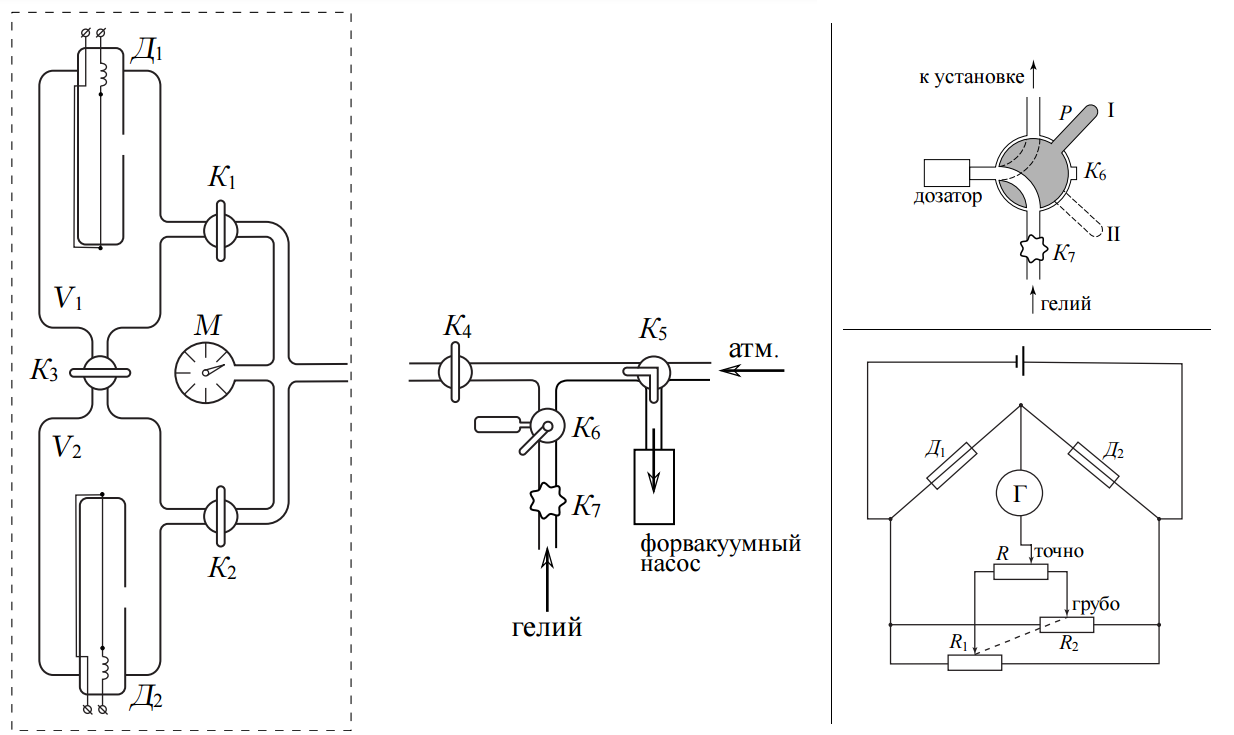
\includegraphics[width=\textwidth]{установка}}
    \caption{Установка}
    \label{установка}
\end{figure}

Здесь $V_1,\; V_2$ -- два сосуда с примерно равным объемом, в которые мы будем загонять воздух и гелий.

Данная конструкция позволяет провести диффузию, которая возможна только при равенстве давлений.

Основное оборудование, с помощью которого мы будем снимать измерения -- датчики теплопроводности, через которые пропускают ток. Они подключены к мосту, который позволяет нам устанавливать начальное равновесное состояние.

При изменении концентрации в колбах вольтметр покажет нам разность напряжений на датчиках, что, из-за их конструкции, означает разность концентраций. 

С помощью изменения напряжения мы и будем изучать процесс диффузии, т.к. во время ее протекания концентрации газов начинают устанавливаться, что заметно на графике разницы напряжений от времени.

% \section{Методика измерений}

% \section{Результаты измерений и обработка данных}

% \section{Обсуждение результатов}

\end{document}
